\documentclass[paper=a4, fontsize=11pt]{scrartcl} % A4 paper and 11pt font size

\usepackage[T1]{fontenc} % Use 8-bit encoding that has 256 glyphs
\usepackage[english]{babel} % English language/hyphenation
\usepackage{amsmath,amsfonts,amsthm} % Math packages
\usepackage{graphicx}

\usepackage{lipsum} % Used for inserting dummy 'Lorem ipsum' text into the template

\usepackage{sectsty} % Allows customizing section commands
\allsectionsfont{\centering \normalfont\scshape} % Make all sections centered, the default font and small caps

\usepackage{fancyhdr} % Custom headers and footers
\pagestyle{fancyplain} % Makes all pages in the document conform to the custom headers and footers
\fancyhead{} % No page header - if you want one, create it in the same way as the footers below
\fancyfoot[L]{} % Empty left footer
\fancyfoot[C]{} % Empty center footer
\fancyfoot[R]{\thepage} % Page numbering for right footer
\renewcommand{\headrulewidth}{0pt} % Remove header underlines
\renewcommand{\footrulewidth}{0pt} % Remove footer underlines
\setlength{\headheight}{13.6pt} % Customize the height of the header

\numberwithin{equation}{section} % Number equations within sections (i.e. 1.1, 1.2, 2.1, 2.2 instead of 1, 2, 3, 4)
\numberwithin{figure}{section} % Number figures within sections (i.e. 1.1, 1.2, 2.1, 2.2 instead of 1, 2, 3, 4)
\numberwithin{table}{section} % Number tables within sections (i.e. 1.1, 1.2, 2.1, 2.2 instead of 1, 2, 3, 4)

\setlength\parindent{0pt} % Removes all indentation from paragraphs - comment this line for an assignment with lots of text

%----------------------------------------------------------------------------------------
%	TITLE SECTION
%----------------------------------------------------------------------------------------

\newcommand{\horrule}[1]{\rule{\linewidth}{#1}} % Create horizontal rule command with 1 argument of height

\title{	
	\normalfont \normalsize 
	\textsc{EC500 - Introduction to Learning From Data} \\ [25pt] % Your university, school and/or department name(s)
	\horrule{0.5pt} \\[0.4cm] % Thin top horizontal rule
	\huge Matlab 3 \\ % The assignment title
	\horrule{2pt} \\[0.5cm] % Thick bottom horizontal rule
}

\author{Mikhail Andreev} % Your name

\date{\normalsize\today} % Today's date or a custom date

\begin{document}
	
	\maketitle % Print the title
	

	%----------------------------------------------------------------------------------------
	%	PROBLEM 1
	%----------------------------------------------------------------------------------------
	
	\newpage
	\section{Exploring Boston Housing Data with Regression Trees}
	The regression tree generated from the training data can be seen here:
	\\\\
	\hspace*{-3cm}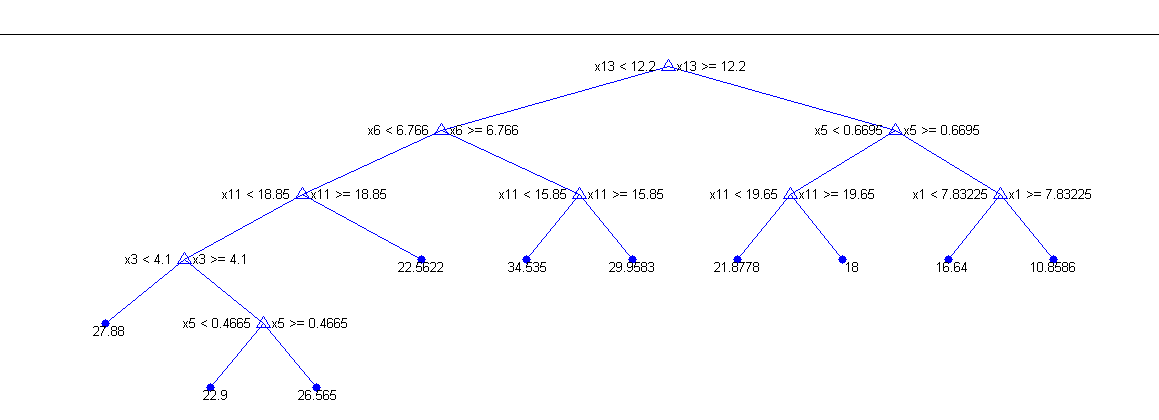
\includegraphics[scale=.7]{tree_diagram}
	\\\\
	Using the input vector:
	\\\\
	$[5, 18, 2.31, 1, 0.5440, 2, 64, 3.7, 1, 300, 15, 390, 10]$
	\\\\
	We get an output $MEDV = 22.047619$.
	\\\\
	If we plot the Mean Absolute Error for both the training and testing sets, using different numbers of observations per leaf, you get the following graph:
	\\\\
	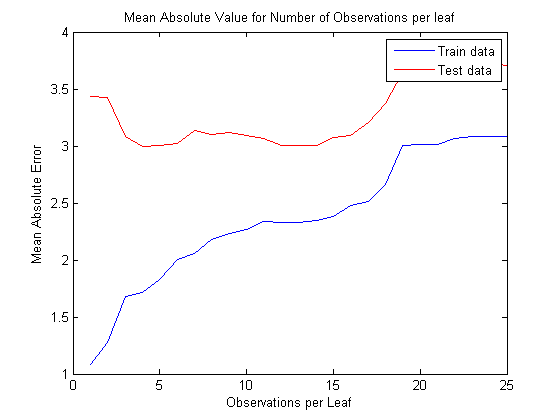
\includegraphics{mae_for_different_observations} 
	\\\\
	From the graph we can see that when the number of observations are low, we essentially memorize the training data, making the training error almost 0, while having a high testing error. As we increase the number of observations, training error starts to steadily increase, while the testing error drops to a lower plateau. For a large number of observations, the testing error is constant, meaning the number of observations is not a deciding factor in the accuracy of the tree in this case. However, after a certain point, each leaf is making too many observations, generalizing the results too much, causing a large increase in both training and testing error.
	\newpage
	\section{Ordinary Least Squares versus Robust Linear Regression}
	When implementing the Ordinary Least Squares method, the input data matrix will in general yield a unique solution. A different input data matrix will return new values of W and b. This occurs because when determining the values of W, they are multiples of the input data matrix.
	\\\\
	The value of $w_{OLS} = 1.2476$. The value of $b_{OLS} = 2.528$. The calculated value of $MSE = 1.390425$. The calculated value of $MAD = 0.965729$.
	\\\\\\
	For cauchy, $MSE = 0.299548$, $MAD = 0.242677$.\\
	For fair, $MSE = 0.286079$, $MAD = 0.246835$.\\
	For huber, $MSE = 0.292181$, $MAD = 0.245091$.\\
	For talwar, $MSE = 0.302416$, $MAD = 0.243493$.\\
	Compared to the above values for OLS, we see the MSE and MAD values are much lower for robustfit. This is due to the fact that robustfit ignores outliers and focus on the majority of proximal points. However, OLS takes everything into account, making an outlier have a large effect on the overall curve.
	\\\\
	The values for huber are: $w_{huber} = 0.127472$, $b_{huber} = 3.094357$.
	\\\\
	We can see the overall graph here:
	\\\\
	\hspace*{-3cm}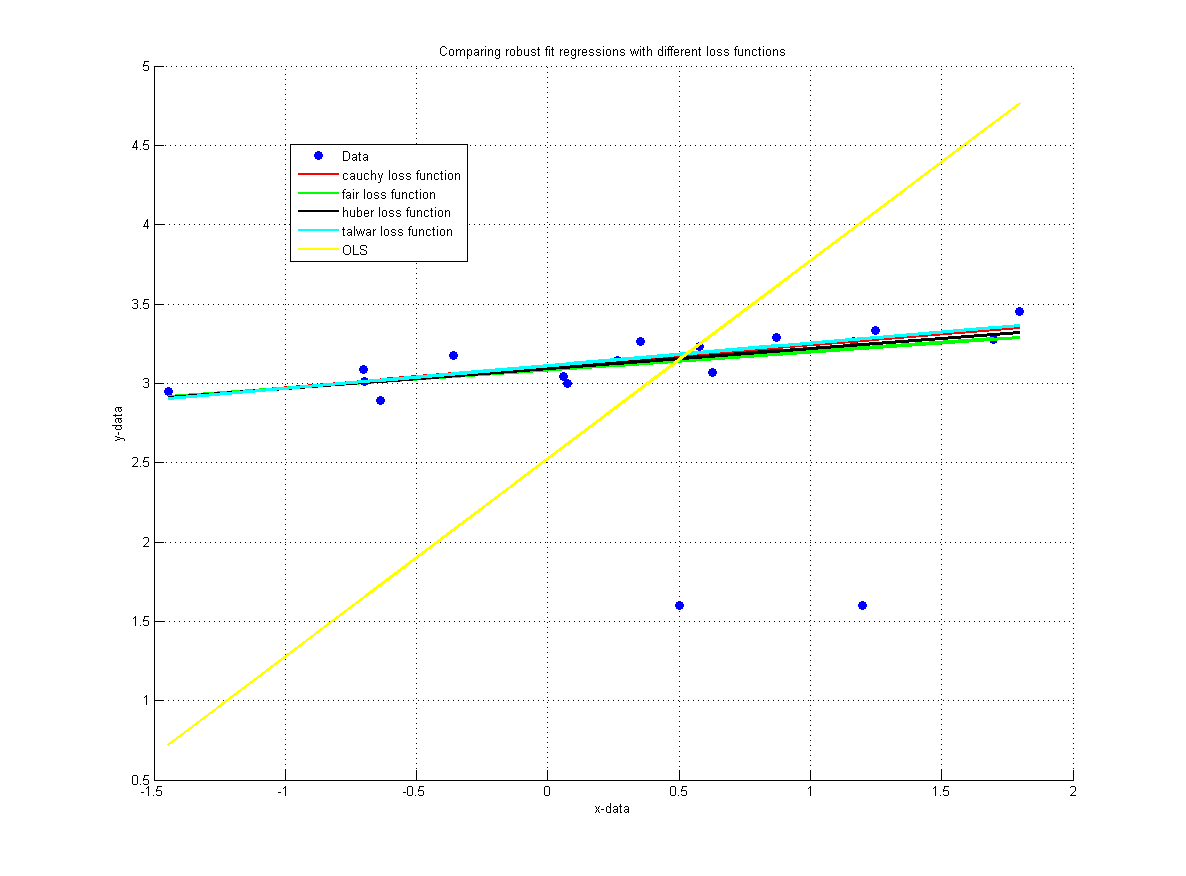
\includegraphics[scale=0.7]{all_methods_graph}
	\\\\
	As mentioned above, we see the 4 robustfit functions are very closely aligned to the majority of points, ignoring outliers. However, OLS is deeply influenced by the outliers, and thus does not make a good fit for the majority of the data.
	
	
	\newpage
	\section{Overfitting and Ridge Regression}
	Here we have the graph for the polynomial regressions of order 2, 6, 10, and 14.
	\\\\
	\hspace*{-3cm}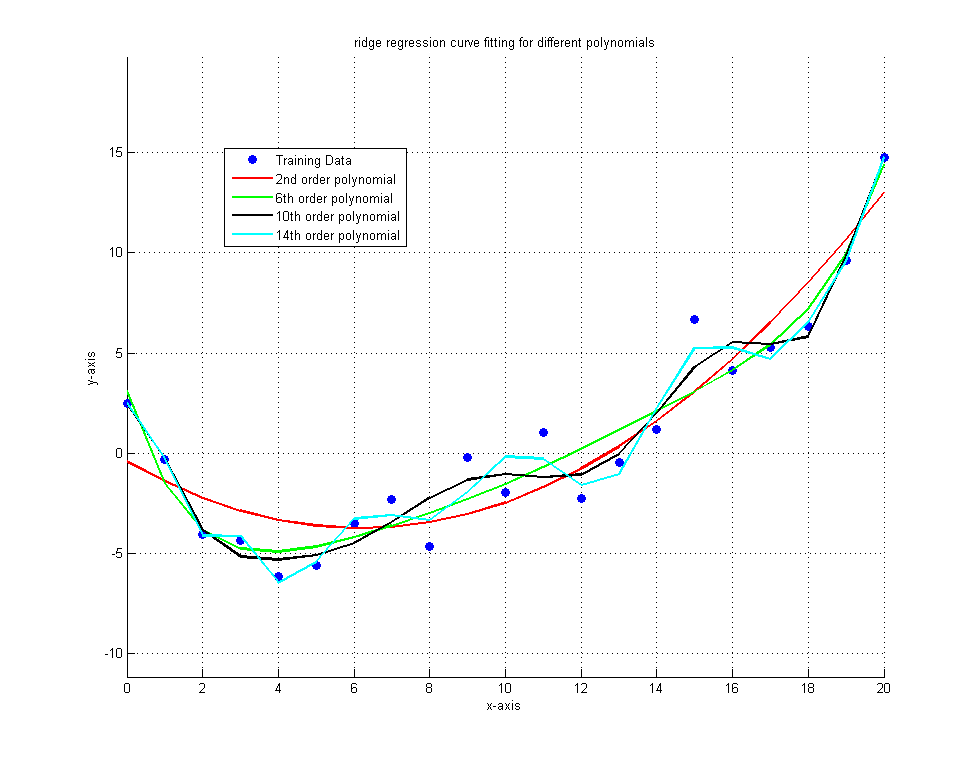
\includegraphics[scale=0.8]{4_order_polynomials}
	\\\\
	From the graph we can see how as the order of the polynomial increases, it fits the data more exactly. This unfortunately also leads to overfitting, so different points will be poorly recognized.
	\\\\
	The following graphs displays the MSE rates for different polynomials on the training and testing sets.
	\\\\
	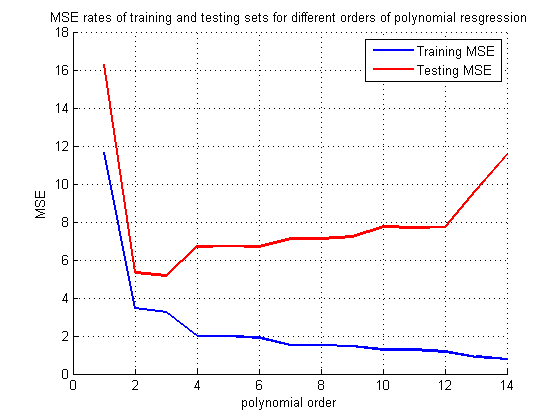
\includegraphics[]{MSE_rates}
	\\\\
	From the graph we can see for the training set, as polynomial order increases, the MSE rate goes down. This is due to overfitting, making the solution fit very closely to the training set, leading to low error. However, because of this our MSE rate for the testing set rises at the same time. Since the data is heavily fitted to the training set, it is not well adapted to the testing set. However, lower order polynomials give lower MSE error since the regression is complex enough to predict the value of the data, but not overfitted.
	\\\\
	The graph for the regularized versus the unregularized regression can be seen here:
	\\\\
	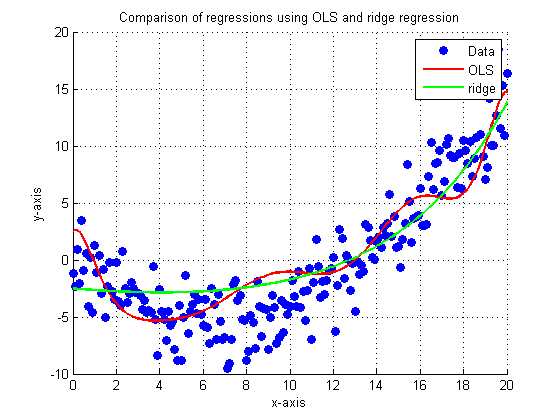
\includegraphics[]{OLS_vs_ridge}
	\\\\
	From this graph we can see that the regularized version is much less curvy, and less overfitted. This allows it to have a better MSE to the testing data.
	\newpage
	\section{Lasso vs Ridge}
	Here we can see the graph for the LASSO coefficients using different $\lambda$:
	\\\\
	\hspace*{-3cm}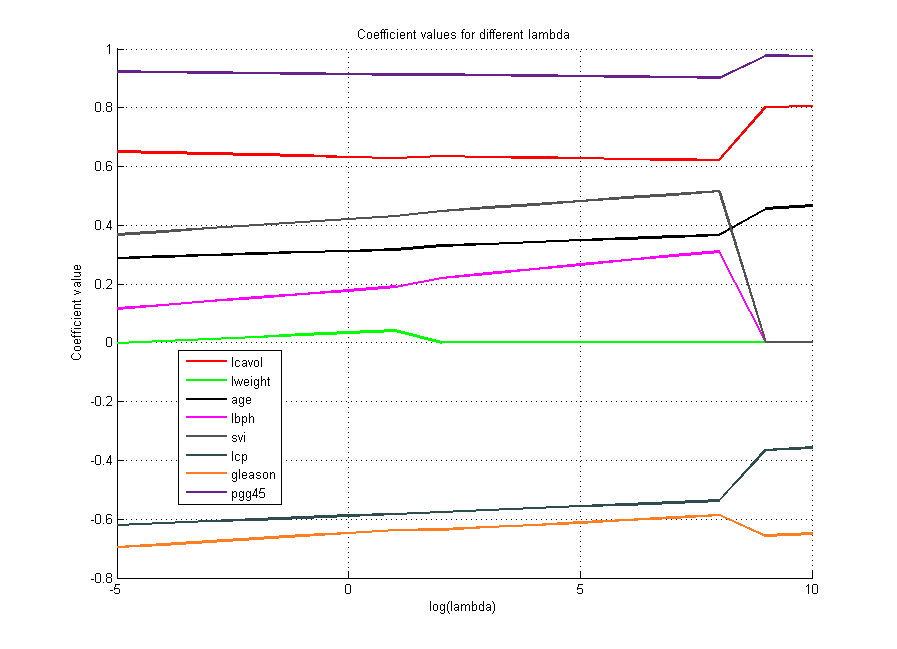
\includegraphics[scale=0.8]{coeff_vs_lambda}
	\\\\
	Using the generated coefficients we can calculate the MSE for each $\lambda$:
	\\\\
	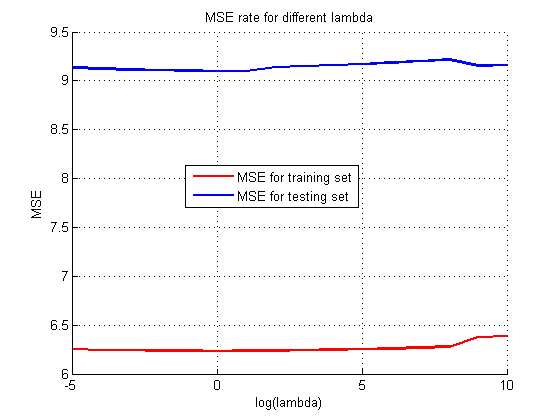
\includegraphics[]{MSE_vs_lambda}
	\\\\
	We can see that as $\lambda$ increases, the coefficients change only slightly, until we get to a $\lambda$ between 7 and 8 which causes a large change in the coefficient value. At the same time we see the MSE rate of the testing set fall slightly, and that of the training set to rise slightly, indicating a large change point in the function. 
	\\\\\\
	The last features to converge are the Gleason score and the percentage Gleason score 4 or 5. This information can be used by giving these features more weight in the regression allowing them to have a larger effect on the outcome. Since they are the more significant, emphasizing them may allow for more accurate prediction.
	\\\\\\
	Using the same method for ridge regression we can get a graph of the coefficients versus $\lambda$:
	\\\\
	\hspace*{-3cm}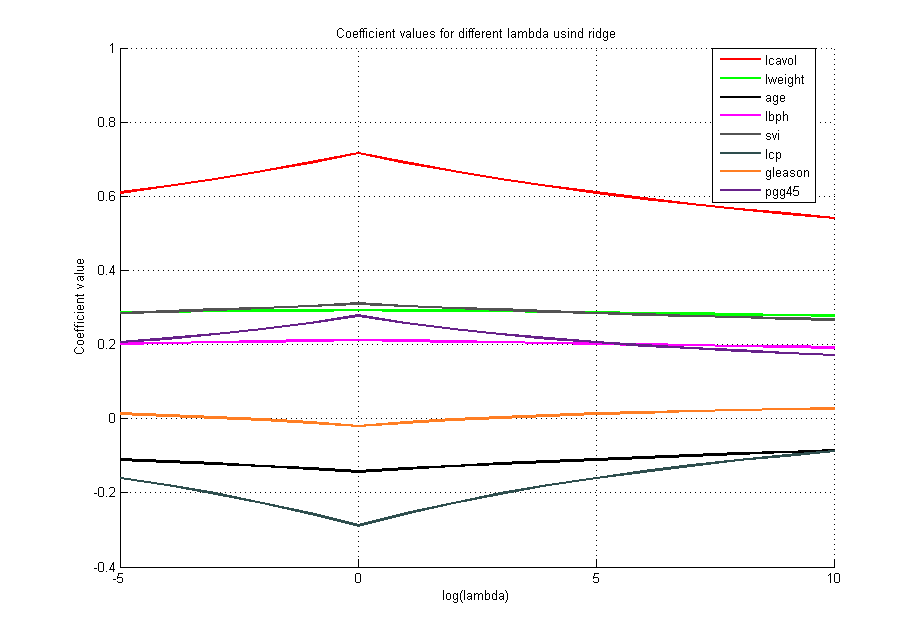
\includegraphics[scale=0.8]{coeff_vs_lambda_ridge}
	\\\\
	And for the MSE rate:
	\\\\
	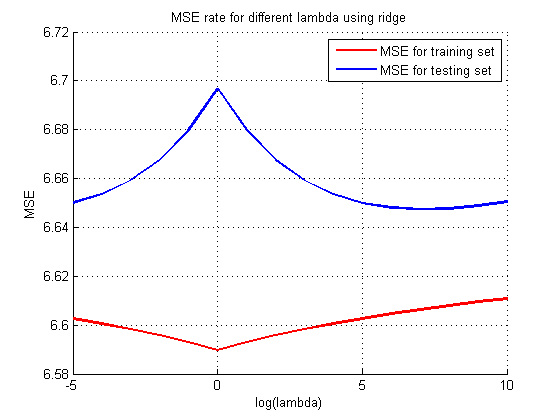
\includegraphics[]{MSE_vs_lambda_ridge}
	\\\\
	From the first graph we can see that unlike lasso regression, ridge regression has the coefficient values highest at $\lambda=0$, and the farther $\lambda$ goes from 0, the closer the coefficients converge to 0. Similarly, the higher the values of the coefficients, the higher the error rate for the testing samples, and the lower the error rate of the training samples. This makes sense since at $\lambda=0$ there is no regularization. Overall, we see far lower error rates in the testing samples using ridge regression than we see in LASSO regression.
	
	
\end{document}